\chapter{Budowa klastra obliczeniowego} \label{ch:budowa-klastra}

W przeszłości głównym zastosowaniem procesorów graficznych było przyspieszanie renderowania
grafiki, głównie w kontekście gier i graficznych interfejsów użytkownika. Wraz z ewolucją
tych układów, rozwinęła się ich zdolność do równoczesnego przetwarzania bardzo dużej liczby
wątków, co pozwala na znaczące przyspieszenie innych aplikacji o~wysokim stopniu równoległości.

Dobrym tego przykładem są nowoczesne układy graficzne, które udostępniają setki, a nawet
tysiące rdzeni dla obliczeń ogólnego przeznaczenia. Dzięki temu są stosunkowo tanim
narzędziem do równoległego przetwarzania danych na wielką skalę \cite{computer-arch}.

Aby zwiększyć wydajność proponowanego klastra względem istniejących rozwiązań, minikomputery
jednopłytkowe będące węzłami wykonawczymi powinny wspierać obliczenia ogólnego przeznaczenia
na układach graficznych (ang. \english{General-Purpose Compute on Graphics Processing Units, GPGPU}).
Szczególnie ważne w tym przypadku jest wsparcie dla popularnych narzędzi do programowania
GPGPU, takich jak CUDA oraz OpenCL.

Aby zapewnić efektywne przechowywanie, transfer i przetwarzanie danych, węzły klastra
powinny posiadać też:
\begin{itemize}
	\item dużą ilość szybkiej pamięci RAM,
	\item szybkie interfejsy dla pamięci trwałej (dyski HDD lub SSD),
	\item karty sieciowe o dużej przepustowości.
\end{itemize}

\section{Porównanie minikomputerów z akceleracją GPU}

Model Raspberry Pi 4, wydany w 2019 roku, przyniósł znaczące ulepszenia pod względem wydajności
w porównaniu do swoich poprzedników. Choć szybsze interfejsy sieciowe, większa ilość pamięci RAM
(nawet do 8 GB) oraz interfejsy USB 3.0 pozwoliły na znaczne zwiększenie wydajności w obliczeniach
\english{Big Data} \cite{rpi-cluster-2}, to brak wsparcia dla technologii CUDA i OpenCL czyni ten
model niewystarczającą podstawą dla węzłów wykonawczych.

Popularnym przedstawicielem minikomputerów jednopłytkowych jest też Intel NUC. Jednostki te
oferują wydajne procesory x86, wbudowane układy graficzne, obsługę szybkich dysków i dużą
rozszerzalność. Komputery NUC są dostępne zarówno w formie gotowych urządzeń, jak i zestawów
do samodzielnego złożenia, co pozwala na dostosowanie ich do konkretnych potrzeb użytkownika.
Najnowsze produkty z tej linii oferują wsparcie dla technologii OpenCL oraz akceleratory
sieci neuronowych, lecz nie wspierają technologii CUDA \cite{nuc-list}.

Nvidia Jetson to kolejna rodzina minikomputerów z akceleracją GPU, początkowo przeznaczona
przede wszystkim do rozwoju aplikacji graficznych 3D. Wkrótce komputery z tej serii stały
się też popularnym narzędziem do prototypowania aplikacji wizji komputerowej, uczenia
maszynowego i Internetu rzeczy.

Swoją popularność zawdzięczają wsparciu technologii CUDA i OpenCL, stosunkowo niskiemu
kosztowi, małym wymiarom oraz obszernemu pakietowi narzędzi Nvidia JetPack SDK.
Biorąc pod uwagę te zalety, do budowy klastra wybrano model Jetson Nano.

Zestaw Jetson Nano Developer Kit wyróżnia się \cite{jetson-spec}:
\begin{itemize}
	\item 128-rdzeniowym procesorem graficznym o maksymalnej wydajności 472 GFLOPS,
	      wspierającym technologie CUDA oraz (nieoficjalnie) OpenCL,
	\item czterordzeniowym procesorem ARM Cortex-A57 o taktowaniu 1.43GHz,
	\item 4 GiB pamięci RAM w technologii LPDDR4, o łącznej przepustowości 25.6 GB/s,
	\item kartą sieciową obsługującą standard Gigabit Ethernet,
	\item obsługą kart pamięci SD, pamięci Flash eMMC i dysków zewnętrznych USB 3 o przepustowości do 5 Gbit/s,
	\item konfigurowalnym poborem mocy (od 5 do 10W),
	\item zasilaniem poprzez port microUSB.
\end{itemize}

\section{Sprzęt i oprogramowanie}

\begin{figure}[h]
	\centering
	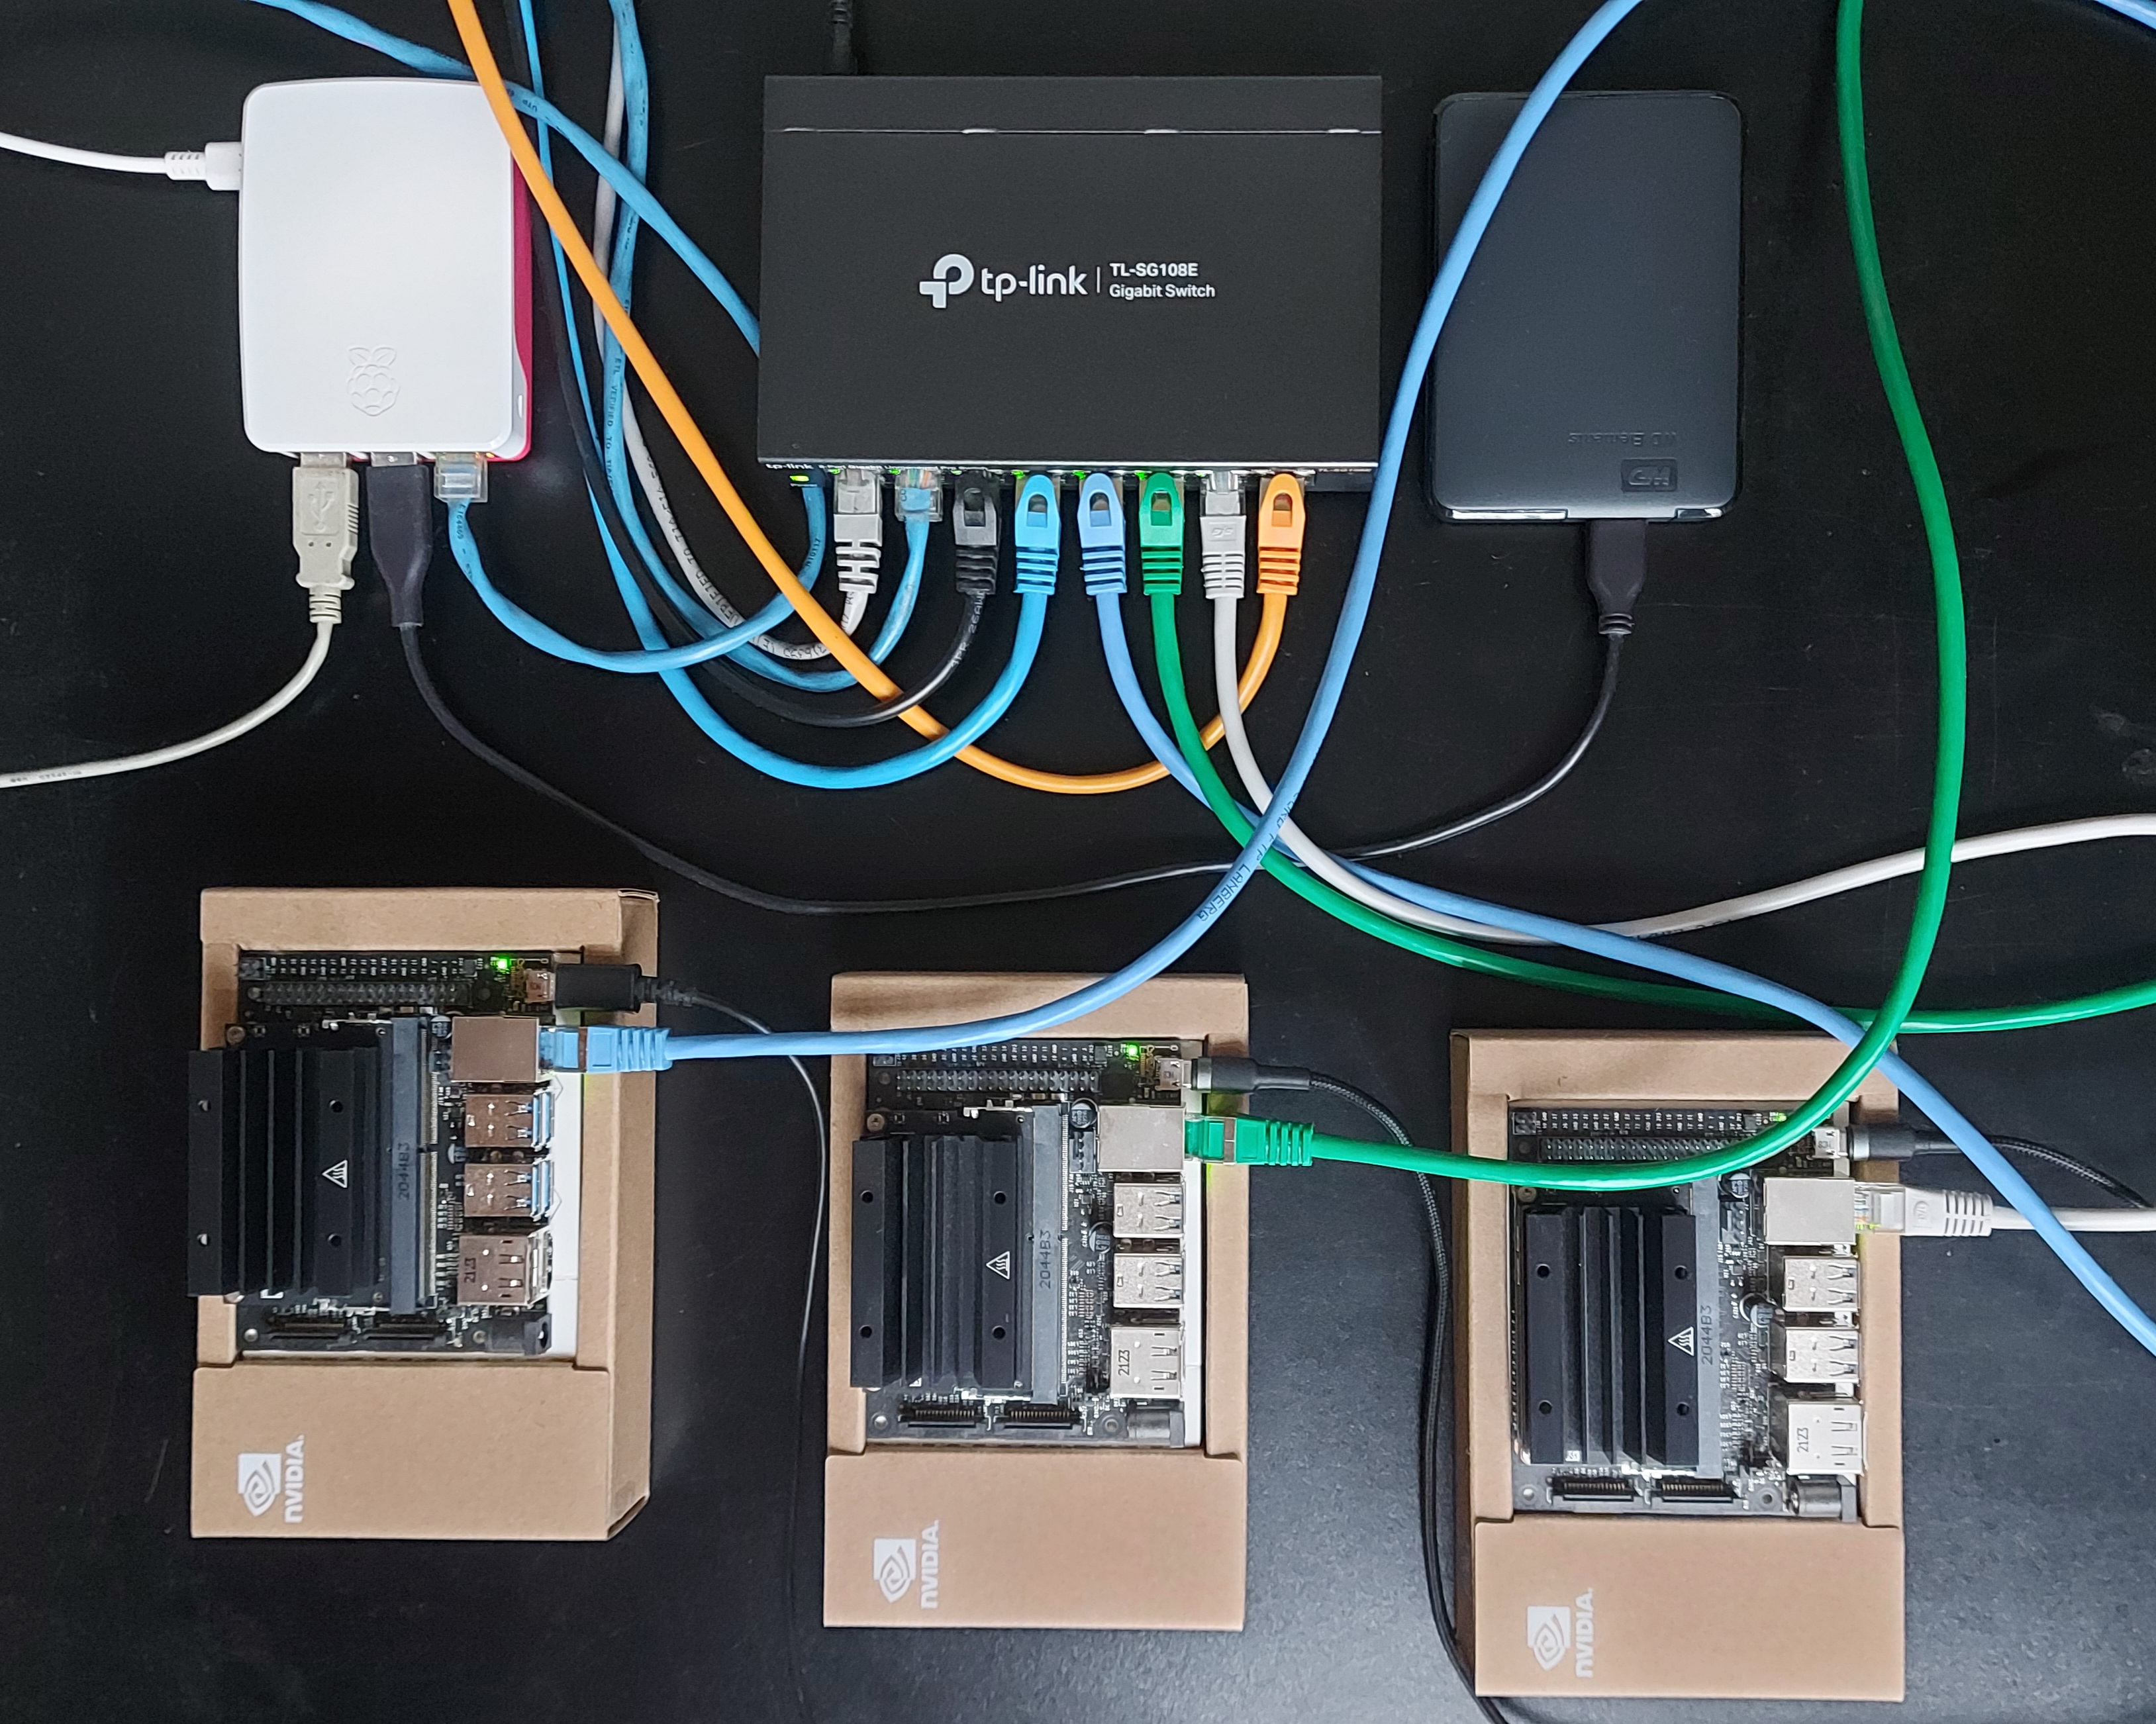
\includegraphics[width=0.7\textwidth]{graf/Cluster-picture.jpg}
	\caption{Klaster minikomputerów zbudowany na potrzeby pracy.}
	\medskip \small
	U góry, kolejno od lewej strony: minikomputer Raspberry Pi 4B, przełącznik sieciowy
	TP-Link oraz dysk zewnętrzny. Na dole widoczne minikomputery Nvidia Jetson Nano.
	\label{pic:cluster-photo}
\end{figure}

Klaster przedstawiony na fotografii \ref{pic:cluster-photo} składa się z czterech węzłów, w tym
jednego węzła nadrzędnego i trzech węzłów wykonawczych. Funkcję węzła nadrzędnego pełni
minikomputer Raspberry Pi 4B w wersji z 2 GB pamięci RAM, który został dodatkowo wyposażony w
dysk twardy USB 3.0 o pojemności 1 TB. Zasilanie minikomputera zapewniane jest przez
zasilacz USB-C dedykowany dla Raspberry Pi.
\newpage

Węzły wykonawcze klastra to minikomputery Nvidia Jetson Nano w wersji z 4 GB pamięci RAM, które
zasilane są przez ładowarkę USB firmy Aukey. Wybrana ładowarka dostarcza maksymalnie 12 W na
każdy z czterech portów, przez co każdy moduł Jetson Nano jest w stanie w pełni wykorzystać
limit poboru mocy.

Rolę dysków dla minikomputerów Jetson Nano pełnią karty microSD SanDisk o~pojemności 16 GB i
klasie szybkości UHS-1. Gwarantują one minimalną szybkość zapisu 10 MB/s i maksymalną
szybkość odczytu do 120 MB/s.

Zgodnie ze schematem przedstawionym na rysunku \ref{fig:cluster-network}, wszystkie węzły
klastra są połączone siecią Gigabit Ethernet poprzez przełącznik sieciowy TP-Link.
Aby ułatwić konfigurację klastra, adresy IP minikomputerów zostały przydzielone statycznie.

\begin{figure}[h]
	\centering
	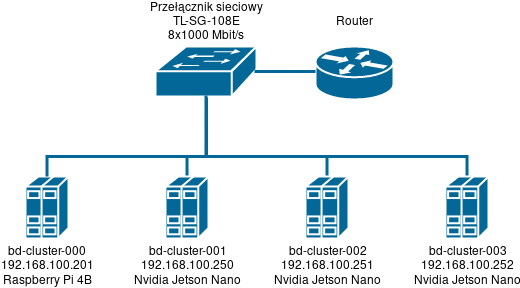
\includegraphics[width=0.6\textwidth]{graf/Cluster-network.png}
	\caption{Schemat sieci komputerowej łączącej węzły klastra.}
	\label{fig:cluster-network}
\end{figure}

Węzeł nadrzędny klastra działa pod kontrolą systemu operacyjnego Ubuntu Server LTS w wersji 20.04.
W przypadku węzłów wykonawczych wykorzystywana jest dystrywbucja Nvidia Jetson Linux w wersji
R32.7.3 (Tab. \ref{tab:software}), która dostarcza sterowniki, biblioteki i narzędzia potrzebne do
rozwoju aplikacji CUDA na platformie Jetson.

Ze względu na brak oficjalnego wsparcia OpenCL dla minikomputera Jetson Nano wykorzystano
otwartą implementację PoCL. Dzięki zastosowaniu projektu LLVM do generacji kodu maszynowego
obsługuje ona wiele architektur, w tym x86, ARM oraz CUDA. Wersja PoCL zawarta w systemie
Jetson Linux domyślnie nie zawiera wsparcia dla architektury CUDA, dlatego też na potrzeby
pracy przygotowano własną kompilację.

Na klastrze zostały zainstalowane platformy Apache Hadoop oraz Apache Spark, a~także wymagane do
ich uruchomienia środowiska OpenJDK 11 i Scala 2.13.

%TC:ignore
\begin{table}[h]
	\centering
	\caption{Wykaz oprogramowania wykorzystanego w badaniach.}
	\begin{tabular}{ | p{7cm} | p{2cm} | p{3cm} | }
		\hline
		Nazwa programu lub biblioteki & Wersja   & Data wydania \\
		\hline
		Nvidia Jetson Linux           & R32.7.3  & 2022-11-22   \\
		Ubuntu Server                 & 20.04.6  & 2023-03-23   \\
		OpenJDK                       & 11.0.19  & 2023-04-18   \\
		Scala                         & 2.13.11  & 2023-06-07   \\
		CUDA Toolkit                  & 10.2.460 & 2021-03-02   \\
		PoCL                          & 3.0      & 2022-06-10   \\
		Apache Hadoop                 & 3.3.5    & 2023-03-22   \\
		Apache Spark                  & 3.4.0    & 2023-04-13   \\
		JCuda                         & 10.2.0   & 2020-02-09   \\
		Aparapi                       & 3.0.0    & 2021-07-12   \\
		Ansible                       & 2.15.5   & 2023-10-09   \\
		\hline
	\end{tabular}
	\label{tab:software}
\end{table}
%TC:endignore

Do implementacji programów testowych wybrano język Java 11, czyli statycznie typowany język
wysokiego poziomu wspierający programowanie obiektowe. Ponieważ jest on wspierany przez obie
platformy obliczeniowe, jego użycie ułatwia ponowne użycie kodu i~konstrukcję programów w
sposób modułowy.

Co więcej, Java jest językiem wieloplatformowym, co oznacza, że napisany i skompilowany kod może
być uruchamiany bez modyfikacji na różnych platformach, od telefonów komórkowych po systemy
mainframe. Programy w języku Java są kompilowane do niezależnego od platformy kodu bajtowego,
który jest następnie interpretowany lub kompilowany do kodu maszynowego przez maszynę wirtualną Javy.

Rysunek \ref{fig:software-stack} przedstawia ogólny widok stosu oprogramowania używanego w~badaniach.
Do wykonywania programów CUDA w programach Java wykorzystano bibliotekę JCuda. Są to bezpośrednie
wiązania do funkcji CUDA w~języku C++, które nie dostarczają dodatkowych warstw abstrakcji. Oprócz
podstawowego interfejsu JCuda używane jest rozszerzenie JCurand. Dostarcza ono wiązania dla
opracowanej przez firmę Nvidia biblioteki cuRAND, która zawiera wydajne implementacje generatorów
liczb losowych w~języku CUDA.

Oprócz generatorów liczb pseudolosowych, cuRAND oferuje też generator oparty o ciągi Sobola, który
cechuje się bardziej równomiernym próbkowaniem przestrzeni wielowymiarowych. Właściwość ta jest
szczególnie ważna w~aplikacjach metody Monte Carlo, ponieważ wpływa korzystnie na dokładność
otrzymywanych wyników.

Niestety, projekt JCuda nie dostarcza gotowych bibliotek natywnych dla architektury ARM,
wykorzystywanej przez minikomputery Jetson Nano. Z tego względu zostały przygotowane własne
kompilacje wymaganych zależności. Na jednym z węzłów klastra skompilowano projekt
\lstinline{jcuda-natives} zawierający komponenty interfejsu natywnego Javy (ang.
\english{Java Native Interface}). Następnie wykorzystując narzędzie Maven zbudowano i~opublikowano
w~\href{https://github.com/users/kmolski/packages?repo_name=masters-thesis}{repozytorium GitHub}
bibliotekę dla języka Java.

Aparapi to kolejna z używanych bibliotek, pozwalająca na wykorzystanie procesorów graficznych w
aplikacjach Java bez konieczności pisania kodu w języku specyficznym dla GPU. Główną zaletą
Aparapi jest zdolność do automatycznej konwersji kodu bajtowego Javy na kod OpenCL w czasie
wykonania. Jeśli program okaże się niemożliwy do przekształcenia, biblioteka automatycznie
cofa się do wykonania kodu na procesorze głównym.

\begin{figure}[h]
	\centering
	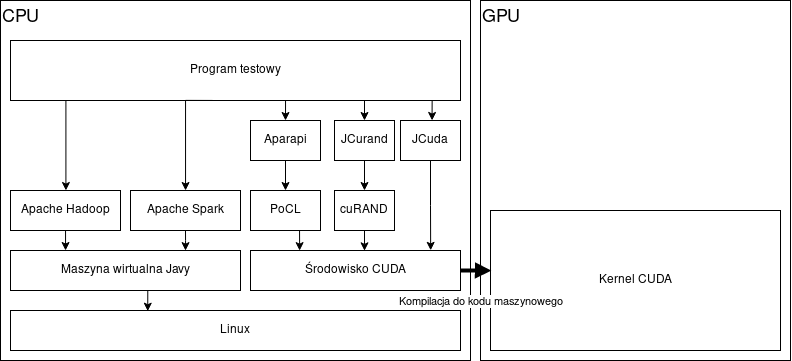
\includegraphics[width=1\textwidth]{graf/Stack.png}
	\caption{Schemat stosu oprogramowania używanego w badaniach.}
	\label{fig:software-stack}
\end{figure}

\section{Proces konfiguracji klastra}

Kluczowym elementem w budowie i ocenie wydajności klastra \english{Big Data} jest nie tylko
wybór odpowiedniego sprzętu, ale także zautomatyzowanie procesów związanych z instalacją
programów oraz konfiguracją środowiska. Zdolność do szybkiej zmiany konfiguracji pozwala na
sprawniejsze przeprowadzenie badań i dokładniejszą ocenę jego wydajności.

Wszystkie komputery zostały skonfigurowane za pomocą Ansible, czyli otwartego narzędzia
do administracji serwerami, zarządzania konfiguracją oraz wdrażania aplikacji.
\newpage

Narzędzie Ansible zostało wybrane ze względu na \cite{ansible-whitepaper}:
\begin{itemize}
	\item modułowość -- Ansible pozwala na organizację zadań w niezależne moduły
	      (nazywane też rolami), co ułatwia ponowne wykorzystanie i tworzenie złożonych zadań,
	\item idempotentność –- wielokrotne zastosowanie skryptów zawsze prowadzi do tego
	      samego stanu docelowego, zapewniając spójność konfiguracji w całym klastrze,
	\item standardowe protokoły -- Ansible komunikuje się z serwerami za pomocą
	      protokołu SSH, którego wsparcie zawarte jest w popularnych systemach operacyjnych,
	\item mechanizm inwentarzy –-  Ansible opisuje zarządzane serwery za pomocą plików w formacie
	      INI lub YAML, nazywanych też inwentarzem. W inwentarzu można tworzyć grupy złożone z
	      serwerów lub innych grup, a także zmienne przypisane do pojedynczego serwera czy grupy,
	\item mechanizm szablonów -- Ansible pozwala na generowanie plików konfiguracyjnych za pomocą
	      języka szablonów Jinja2, wspierającego użycie zmiennych, instrukcji warunkowych i pętli,
	\item wsparcie dla różnych platform –- Ansible działa na wszystkich popularnych
	      systemach operacyjnych i architekturach sprzętowych.
\end{itemize}

Ręczna część konfiguracji klastra ogranicza się do instalacji systemu operacyjnego
Jetson Linux. Po wgraniu obrazu systemu na kartę microSD i włączeniu minikomputera
uruchamiany jest instalator graficzny, w którym należy wykonać następujące czynności:
\begin{enumerate}
	\item Skonfigurować połączenie sieciowe oraz statyczny adres IP;
	\item Utworzyć konto użytkownika z hasłem;
	\item Wybrać tryb zarządzania energią "MAXN".
\end{enumerate}

Po zakończeniu pracy instalatora należy dodać statyczne adresy IP urządzeń do inwentarza
Ansible, a następnie za pomocą programu \lstinline{ansible-playbook} uruchomić kolejno
skrypty \lstinline{setup-os.yaml}, \lstinline{setup-pocl.yaml},
\lstinline{setup-hadoop.yaml} oraz \lstinline{setup-spark.yaml}.

\subsection*{Skrypty Ansible i narzędzia administracyjne}

W ramach pracy utworzono projekt Ansible, którego zadaniem jest automatyzacja procesów instalacji
programów oraz konfiguracji klastra. Skrypty Ansible wchodzące w~skład projektu zapewniają
niezawodność i powtarzalność procesów przy jednoczesnym zachowaniu czytelności
i łatwości użycia.

Kluczowym elementem każdego projektu Ansible jest inwentarz, który opisuje zbiór serwerów, na
którym mają zostać wykonane skrypty. W przypadku wspomnianego projektu inwentarz definiuje
statyczne adresy IP komputerów, podział węzłów na nadrzędne i wykonawcze, konfigurację
klienta Git, a także wersje instalowanych programów.

Kolejną częścią projektu są skrypty, które określają serię zadań do wykonania na węzłach
klastra. Zawierają one konkretne instrukcje opisane poniżej:
\begin{itemize}
	\item \lstinline{setup-os.yaml} -- przeprowadzenie wstępnej konfiguracji i aktualizacji systemu. \newline
	      Wyłączany jest tryb graficzny i ograniczenie czasu wykonania dla kerneli CUDA,
	\item \lstinline{setup-pocl.yaml} -- instalacja własnej kompilacji biblioteki PoCL,
	      dostarczającej nieoficjalne wsparcie OpenCL dla procesora graficznego w komputerze Jetson Nano,
	\item \lstinline{setup-hadoop.yaml} -- instalacja i konfiguracja platformy Apache Hadoop. \newline
	      W ramach tego skryptu formatowany jest też system plików HDFS,
	\item \lstinline{setup-spark.yaml} -- instalacja i konfiguracja platformy Apache Spark. \newline
	      W tym skrypcie instalowany jest również język programowania Scala.
\end{itemize}

Aby zwiększyć modułowość projektu, zgrupowano w role następujące zadania:
\begin{itemize}
	\item \lstinline{includes/updated} -- zadania związane z aktualizacją systemu operacyjnego,
	\item \lstinline{roles/common-tools} -- zadania do instalacji środowiska Java, konfiguracji
	      nazwy hosta, strefy czasowej oraz klienta Git,
	\item \lstinline{roles/security-config} -- konfiguracja zabezpieczeń usługi SSH.
\end{itemize}

Wykorzystując dane zawarte w inwentarzu i mechanizm szablonów udostępniany przez Ansible, skrypty
instalacyjne generują dla klastra następujące pliki konfiguracyjne:
\begin{itemize}
	\item \lstinline{core-site.xml} -- główna konfiguracja Hadoop, zawiera adres klastra HDFS,
	\item \lstinline{environment} -- konfiguracja zmiennej \lstinline{PATH}, służącej do lokalizacji programów,
	\item \lstinline{hdfs-site.xml} -- konfiguracja klastra HDFS zawierająca ustawienia replikacji danych,
	\item \lstinline{mapred-site.xml} -- konfiguracja komponentu MapReduce dla platformy Hadoop,
	\item \lstinline{yarn-site.xml} -- ustawienia menedżera zasobów YARN,
	\item \lstinline{workers} -- lista węzłów wykonawczych dla platformy Hadoop,
	\item \lstinline{spark-env.sh} -- konfiguracja platformy Spark do działania w trybie samodzielnym,
	\item \lstinline{slaves} -- lista węzłów wykonawczych dla platformy Spark.
\end{itemize}

Oprócz zadań administracyjnych, automatyzacji podlega także uruchamianie programów
testowych i zbieranie informacji o wydajności. Zapewnia to lepszą powtarzalność
pomiarów, a co za tym idzie -- większą przejrzystość i weryfikowalność badań.
Dlatego też do automatyzacji często wykonywanych zadań utworzono skrypty w języku Bash:
\begin{itemize}
	\item \lstinline{bench-*.sh} --
	      uruchamianie programów testowych dla wszystkich kombinacji
	      parametrów i danych wejściowych,
	\item \lstinline{start-hadoop.sh} i \lstinline{stop-hadoop.sh} --
	      uruchamianie i zamykanie platformy Apache Hadoop wraz z~systemem plików HDFS,
	\item \lstinline{start-spark.sh} i \lstinline{stop-spark.sh} --
	      uruchamianie i zamykanie platformy Apache Spark wraz z~systemem plików HDFS,
	\item \lstinline{clear-hdfs-out.sh} i \lstinline{clear-hdfs-tmp.sh} --
	      usuwanie plików wynikowych i plików tymczasowych programów,
	\item \lstinline{report-perf.sh} -- odczytywanie miar wydajności z
	      plików dziennika utworzonych przez programy testowe.
\end{itemize}

\section{Programy testowe}

Do badań wydajności klastra przygotowano zadania rozproszone w języku Java, które wykorzystują
platformy obliczeniowe Apache Hadoop i Apache Spark. Wszystkie programy testowe wspierają wykonanie
zarówno na procesorze głównym, jak i graficznym przy użyciu technologii CUDA. Jeden z algorytmów
został też zrealizowany przy użyciu standardu OpenCL.

Zestaw programów testowych składa się zarówno ze zmodyfikowanych wersji przykładów z dystrybucji
Hadoop oraz Spark, jak i nowych programów stworzonych na potrzeby pracy. Aby kompleksowo
ocenić wydajność klastra oraz opłacalność wykorzystania GPU w obliczeniach \english{Big Data},
zestaw testowy zawiera aplikacje o różnych charakterystykach użycia dysku i procesora.

Projekt zawierający programy testowe jest zarządzany przez Apache Maven, czyli narzędzie do
zarządzania projektami opartymi o język Java. Maven automatyzuje wiele etapów tworzenia
oprogramowania, takich jak kompilacja, testowanie, generowanie dokumentacji oraz budowanie
paczek JAR (ang. \english{Java ARchive}). Co więcej, centralne repozytorium Maven udostępnia
programistom wiele bibliotek dla języka Java, które mogą być dodawane do projektu poprzez
prostą zmianę konfiguracji.

Programy testowe zostały podzielone przy użyciu modułów Maven, czyli podprojektów wchodzących
w skład jednego projektu nadrzędnego. Moduły są kompilowane jako niezależne jednostki,
które mogą definiować zależności między sobą. Na przykład, moduł interfejsu konsolowego może
zależeć od modułu zawierającego logikę aplikacji.

Implementacje programów testowych zostały podzielone na trzy moduły:
\begin{itemize}
	\item moduł \lstinline{common} -- częściowe implementacje algorytmów w językach
	      Java oraz CUDA, funkcje ułatwiające wykonywanie programów CUDA i obsługę zasobów,
	\item moduł \lstinline{hadoop-benchmark} -- funkcje pomocnicze do zarządzania zadaniami w Apache Hadoop,
	      implementacje programów PiEstimation, FuzzyGen, FuzzyCompute oraz FuzzyFilter dla platformy Hadoop,
	\item moduł \lstinline{spark-benchmark} -- funkcje pomocnicze do zarządzania kontekstem w Apache Spark,
	      implementacje progrmaów PiEstimation, FuzzyGen, FuzzyCompute oraz FuzzyFilter dla platformy Spark.
\end{itemize}

Projekt nadrzędny może zawierać wspólną konfigurację, która może być następnie używana we
wszystkich modułach. Na przykład, zamiast określać wersje bibliotek w każdym module
osobno, można to zrobić jednokrotnie w nadrzędnym projekcie, co ułatwia aktualizację
zależności i zapewnia spójność ich wersji.

Maven posiada też wsparcie dla wtyczek, które umożliwiają dostosowywanie procesu budowy do
indywidualnych potrzeb projektu. W przypadku programów testowych wykorzystywane są wtyczki do
wykonywania narzędzia Make (wtyczka \lstinline{exec-maven-plugin}) oraz tworzenia obrazów aplikacji
wraz z wymaganymi do uruchomienia bibliotekami (wtyczka \lstinline{maven-assembly-plugin}).

\subsection{Program PiEstimation}

Pierwszym programem testowym jest PiEstimation, który wykorzystuje metodę Monte Carlo do szacowania
wartości liczby $\pi$. Wersja dla procesora głównego to rozwinięcie programu QuasiMonteCarlo
zawartego w oficjalnej dystrybucji Apache Hadoop, a jej odpowiedniki dla procesora graficznego
to autorskie konwersje w językach CUDA oraz OpenCL.

Metoda Monte Carlo to metoda numeryczna stosowana do rozwiązywania problemów poprzez próbkowanie
losowe. Oznacza to, że przeprowadzana jest symulacja wielu prób (lub "eksperymentów") w celu uzyskania
rozkładu wyników, których średnia może być następnie użyta do oszacowania oczekiwanej wartości rozwiązania.

Warianty tej metody są stosowane w wielu dziedzinach nauki, takich jak fizyka, matematyka, finanse,
czy medycyna. Jej przykładowe zastosowania to obliczanie wartości całek, szacowanie wartości
oczekiwanej, optymalizacja funkcji, symulacja sieci, symulacja zdarzeń dyskretnych i wiele innych.

Szacowanie liczby $\pi$ za pomocą metody Monte Carlo to klasyczny przykład zastosowania tej techniki.
Wykonuje się w nim losowe próbkowanie punktów wewnątrz kwadratu i określa ich położenie względem
wpisanego w ten kwadrat koła, co ilustruje rysunek \ref{fig:monte-carlo}.

\begin{figure}[h]
	\centering
	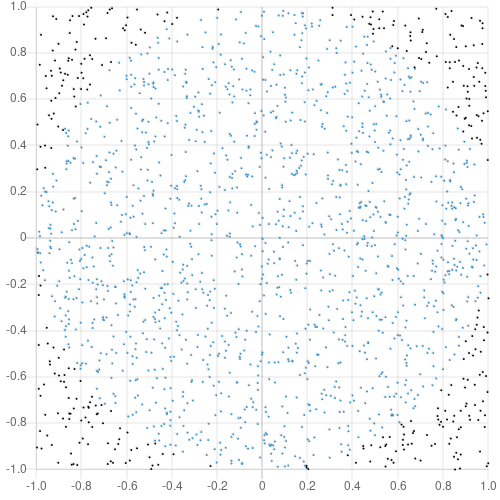
\includegraphics[width=0.8\textwidth]{graf/Pi-estimation.png}
	\caption{Rozkład wartości losowych używany do estymacji liczby $\pi$.}
	\medskip \small
	Czarne punkty znajdują się poza kołem, a punkty niebieskie -- wewnątrz koła.
	\label{fig:monte-carlo}
\end{figure}

\subsubsection*{Implementacja metody Monte Carlo}

Rozważmy kwadrat o boku długości 2, którego środek znajduje się w punkcie (0,0). W ten kwadrat wpisywane
jest koło o promieniu 1, również o środku w punkcie (0,0). Powierzchnia kwadratu wynosi więc 4, a
powierzchnia koła jest równa $\pi$.

Następnie wybieramy losowo punkty o losowych współrzędnych X i Y z zakresu [-1, 1], czyli znajdujących
się wewnątrz kwadratu. Dla każdego punktu sprawdzamy, czy leży on wewnątrz koła. Robimy to, obliczając
jego odległość od środka kwadratu (i koła) za pomocą wzoru \(d = x^2 + y^2\). Jeśli odległość
jest mniejsza lub równa 1, punkt leży wewnątrz koła, a w przeciwnym razie leży poza nim.

Po przeprowadzeniu wielu takich prób obliczamy stosunek liczby punktów wewnątrz koła do
całkowitej liczby punktów wewnątrz kwadratu. Wraz ze zwiększającą się liczbą wybranych
punktów stosunek punktów wewnątrz okręgu do punktów wewnątrz kwadratu będzie coraz
bardziej zbliżony do stosunku ich powierzchni, czyli \(\pi / 4\).

Programy komputerowe realizujące metodę Monte Carlo najczęściej używają generatora liczb
pseudolosowych, którego jakość, wraz z liczbą wybranych punktów, jest głównym czynnikiem
wpływającym na dokładność wyniku.

Użyty w programie generator liczb pseudolosowych oparty jest o ciąg Haltona, czyli
technikę generowania ciągów opartą o rozwinięcia w systemach liczbowych o różnych podstawach.
W przeciwieństwie do tradycyjnych sekwencji losowych sekwencje te zapewniają bardziej
jednolite próbkowanie przestrzeni, co ogranicza błąd obliczeń \cite{monte-carlo}.

Algorytm generacji punktów z użyciem sekwencji Haltona jest nastepujący:
\begin{enumerate}
	\item Dla każdego wymiaru wybierz unikalną liczbę pierwszą \( p \),
	\item Dla każdej liczby pierwszej \( p \) i kolejnych liczb \( i \),
	      wygeneruj rozwinięcia liczb \( i \) o~podstawie \( p \),
	\item Przekształć rozwinięcia liczb \( i \) na wartość ułamkową, aby uzyskać
	      elementy sekwencji dla tej podstawy,
	\item Połącz powstałe sekwencje w celu uzyskania wielowymiarowych punktów.
\end{enumerate}

Ponieważ wartości generowane przez sekwencję są stałe i zależą tylko od podstaw sekwencji,
testowanie implementacji w różnych językach sprowadzało się do porównania końcowych wyników.

Program dla platformy Hadoop wykorzystuje następujące komponenty \english{Mapper},
które zostały opisane w załączniku \ref{ch:techdoc}:
\begin{itemize}
	\item CpuQmcMapper (listing \ref{ch:cpu-qmc-mapper}) -- implementacja dla procesora głównego,
	\item AparapiQmcMapper (listing \ref{ch:aparapi-qmc-mapper}) -- implementacja w języku Java wykorzystująca bibliotekę Aparapi i OpenCL,
	\item JcudaQmcMapper (listing \ref{ch:jcuda-qmc-mapper}) -- implementacja algorytmu w języku CUDA.
\end{itemize}

Ich odpowiednikami dla platformy Spark są klasy CpuQmcFunction, AparapiQmcFunction oraz JcudaQmcFunction (listingi \ref{ch:cpu-qmc-function}, \ref{ch:aparapi-qmc-function} oraz
\ref{ch:jcuda-qmc-function}).

\subsubsection*{Specyfikacja zewnętrzna}

Programy dla platform Apache Hadoop oraz Apache Spark oczekują trzech argumentów wiersza poleceń:
\begin{itemize}
	\item \lstinline{nMaps} -- liczba niezależnych zadań używanych w estymacji,
	\item \lstinline{nSamples} -- liczba próbek przetwarzanych w jednym zadaniu,
	\item \lstinline{mapper} -- implementacja algorytmu (jedna z wartości "cpu", "opencl" lub "cuda").
\end{itemize}

Program wyświetla w konsoli liczbę próbek, algorytm, czas wykonania oraz oszacowaną wartość liczby $\pi$, co przedstawiono na rysunku \ref{fig:piestimation:run}.
Jeśli argumenty nie zostały dostarczone lub są nieprawidłowe, aplikacja wyświetli komunikat o
błędzie wraz z instrukcją poprawnego użycia.

\begin{figure}[h]
	\centering
	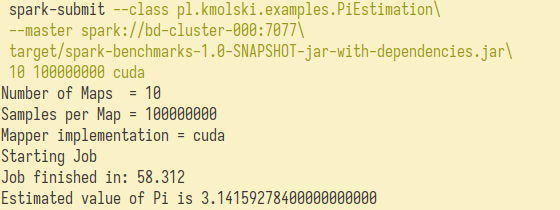
\includegraphics[width=0.8\textwidth]{graf/PiEstimation-interface.png}
	\caption{Przykładowe wywołanie programu PiEstimation.}
	\label{fig:piestimation:run}
\end{figure}

Aplikacja dla platformy Hadoop zapisuje pliki tymczasowe w katalogach \lstinline{/tmp} i \lstinline{/out}
systemu plików HDFS, które są usuwane po zakończeniu zadania.

\subsection{Program FuzzyGen}

Zadaniem kolejnego programu testowego jest generowanie zbiorów danych o różnej objętości dla programu
FuzzyCompute. Dane programu FuzzyCompute składają się z~wielu porcji, z~których każda zawiera 64
zbiory. Każdy zbiór zawiera stopnie przynależności dla 4 rekordów, w~zakresie od 0 do 1.

Porcje danych są zapisywane jako pliki binarne w formacie SequenceFile, dostarczanym przez platformę
Hadoop. Pliki SequenceFile przechowują pary klucz-wartość w skompresowanej formie, co pozwala
zmniejszyć zapotrzebowanie na przestrzeń dyskową i~zwiększyć efektywną szybkość systemu plików.

Algorytm dla procesora głównego wykorzystuje generator liczb losowych z biblioteki standardowej języka Java,
który jest oparty o liniowe generatory kongruentne. Generator ten jest oparty o deterministyczny algorytm i
zapewnia stosunkowo dobrą wydajność, nie jest jednak odpowiedni do zastosowań kryptograficznych.

Wersja algorytmu dla procesora graficznego wykorzystuje bibliotekę JCurand, która udostępnia
funkcjonalność biblioteki cuRAND w języku Java. Biblioteka cuRAND jest z kolei częścią zestawu narzędzi
deweloperskich CUDA, dostarczającą funkcje do generowania liczb losowych na procesorach graficznych
firmy NVIDIA.
\newpage

cuRAND oferuje kilka typów generatorów liczb pseudolosowych, są to między innymi:
\begin{itemize}
	\item generator XORWOW,
	\item generator MRG32K3A,
	\item generator Mersenne Twister (MT19937),
	\item generator Philox 4x32.
\end{itemize}

Za pomocą generatorów cuRAND możliwe jest generowanie liczb dla różnych rozkładów prawdopodobieństwa,
takich jak rozkład Poissona, jednostajny lub normalny.

Program Hadoop wykorzystuje następujące klasy komponentów \english{Mapper},
które zostały opisane w załączniku \ref{ch:techdoc}:
\begin{itemize}
	\item CpuFuzzyGenMapper (listing \ref{ch:cpu-fuzzygen-mapper}) -- algorytm dla procesora głównego,
	\item JcudaFuzzyGenMapper (listing \ref{ch:jcuda-fuzzygen-mapper}) -- algorytm używający funkcji z biblioteki JCurand.
\end{itemize}

W programie dla Apache Spark wykorzystywane są klasy CpuFuzzyGenFunction i~JcudaFuzzyGenFunction (listingi \ref{ch:cpu-fuzzygen-function} oraz \ref{ch:jcuda-fuzzygen-function}).

\subsubsection*{Specyfikacja zewnętrzna}

Aplikacje dla Apache Hadoop oraz Apache Spark oczekują trzech argumentów wiersza poleceń:
\begin{itemize}
	\item \lstinline{mapper} -- definiujący wykorzystywany algorytm (do wyboru: "cpu" lub "cuda"),
	\item \lstinline{nRecords} -- liczba porcji danych do wygenerowania,
	\item \lstinline{outputDir} -- katalog HDFS, w którym zostaną zapisane pliki wynikowe.
\end{itemize}

Program wyświetla w konsoli liczbę porcji danych, algorytm oraz czas wykonania, co przedstawiono
na rysunku \ref{fig:fuzzygen:run}. Gdy wymagane argumenty nie zostaną podane lub są błędne,
program pokazuje komunikat o~błędzie oraz instrukcję prawidłowego użycia.

\begin{figure}[h]
	\centering
	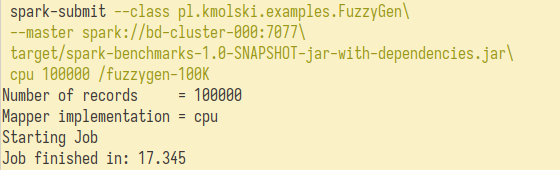
\includegraphics[width=0.8\textwidth]{graf/FuzzyGen-interface.png}
	\caption{Przykładowe wywołanie programu FuzzyGen.}
	\label{fig:fuzzygen:run}
\end{figure}

Zarówno program dla platformy Hadoop, jak i~odpowiednik dla platformy Spark zapisuje dane
wyjściowe w formacie SequenceFile bez użycia kompresji. Zadanie Hadoop definiuje tylko
etap \english{Map}, przez co pliki wynikowe są zapisywane w kilku częściach.

\subsection{Program FuzzyCompute}

Kolejny program jest testem wydajności dla operacji wykonywanych na zbiorach rozmytych.
Zbiory rozmyte stanowią centralny element logiki rozmytej i zostały zdefiniowane przez
Lotfi Zadeha jako rozwinięcie tradycyjnej teorii zbiorów. Umożliwiają one reprezentację
niejasności i wieloznaczności w klasyfikacji obiektów \cite{fuzzy-sets}.

Zbiory rozmyte znalazły szerokie zastosowanie w różnych dziedzinach, takich jak sterowanie
rozmyte, systemy ekspertowe, analiza ryzyka oraz przetwarzanie obrazów. Znacząco ułatwiają
one modelowanie sytuacji, w których granice decyzyjne są trudne do określenia.

W klasycznej teorii zbiorów element albo należy do zbioru (i ma przynależność równą 1),
albo do niego nie należy (i ma przynależność równą 0). W zbiorach rozmytych stopień
przynależności elementu jest opisany przez funkcję przynależności, która przyjmuje wartość
liczbową w zakresie od 0 do 1.

Rozważmy zbiór przedmiotów pochodzących z różnych epok. Używając klasycznej teorii zbiorów,
możemy określić jedynie to, że dany przedmiot albo jest antykiem, albo nim nie jest. Jeśli
wiek przedmiotu znajdzie się tuż pod przyjętym progiem, to zostanie sklasyfikowany jako nie-antyk.

Jeżeli jednak opiszemy te same przedmioty za pomocą zbiorów rozmytych, możemy uzyskać bardziej
użyteczną klasyfikację. Przykładowo, funkcja przedstawiona na rysunku \ref{fig:fuzzy-fn} przypisuje
20-letni przedmiot do zbioru antyków z przynależnością 0, 250-letni -- z~przynależnością 0.5, a
500-letni -- z przynależnością wynoszącą 1.

\begin{figure}[h]
	\centering
	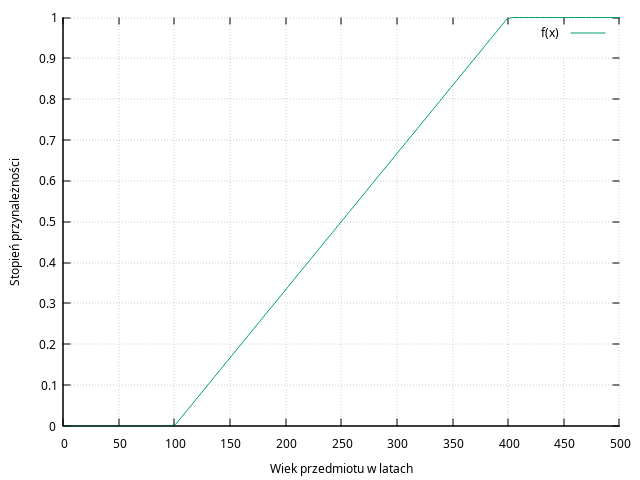
\includegraphics[width=0.6\textwidth]{graf/Fuzzy-membership.png}
	\caption{Wykres przykładowej funkcji przynależności dla zbioru rozmytego.}
	\label{fig:fuzzy-fn}
\end{figure}

Podobnie jak w klasycznej teorii zbiorów, na zbiorach rozmytych definiowane są różne operacje,
takie jak suma, iloczyn, czy dopełnienie. Podczas gdy koncepcja tych operacji pozostaje podobna,
ich realizacje różnią się od tych znanych z klasycznej teorii zbiorów, ponieważ uwzględniają
rozmyte podejście do przynależności.

Suma zbiorów rozmytych może być zdefiniowana jako maksimum stopni przynależności każdego elementu do
obu zbiorów. Niech \(A\) i \(B\) będą zbiorami rozmytymi w przestrzeni \(X\) z funkcjami
przynależności odpowiednio \(\mu A\) i \(\mu B\). Suma zbiorów \(A\) i \(B\) jest zbiorem rozmytym
\(C\) z funkcją przynależności \(\mu C\), która jest definiowana następująco dla każdego elementu
w przestrzeni \(X\) za pomocą wzoru \ref{eq:fuzzy-sum}.

\begin{equation}
    \mu C(x) = max(\mu A(x), \mu B(x))
    \label{eq:fuzzy-sum}
\end{equation}

Dla każdego elementu \(x\) stopień przynależności do sumy \(C\) jest większym z dwóch stopni
przynależności do zbiorów \(A\) i \(B\). Taką operację binarną, używaną do modelowania operacji
"lub" w kontekście zbiorów rozmytych, nazywamy T-konormą lub S-normą. Do S-norm można zaliczyć
też sumę algebraiczną, sumę drastyczną, czy sumę Łukasiewicza.

Dopełnienie zbioru rozmytego polega na odwróceniu stopnia przynależności każdego elementu w
danym zbiorze rozmytym. Jeśli mamy zbiór rozmyty \(A\) na przestrzeni uniwersalnej \(X\) z
funkcją przynależności \(\mu A\), dopełnienie tego zbioru, oznaczone jako \(A'\) lub \(\lnot A\),
ma funkcję przynależności \(\mu A'\) określoną dla każdego elementu \(x\) z \(X\)
wzorem \ref{eq:fuzzy-compl}.

\begin{equation}
    \mu A'(x) = 1 - \mu A(x)
    \label{eq:fuzzy-compl}
\end{equation}

Aplikacje dla platform Hadoop oraz Spark przetwarzają podziały zbiorów wygenerowanych przez program
FuzzyGen. Składają się one z 64 zbiorów, z~których każdy zawiera cztery liczby losowe z~zakresu od
0 do 1. Po wczytaniu zbiorów rozmytych, do zbioru danych dodawane są ich dopełnienia.
Następnie wszystkie zbiory rozmyte są sumowane krzyżowo, co zwiększa złożoność obliczeniową programu.

Aplikacja dla platformy Hadoop wykorzystuje następujące komponenty \english{Mapper},
które zostały opisane w załączniku \ref{ch:techdoc}:
\begin{itemize}
	\item CpuFuzzyComputeMapper (listing \ref{ch:cpu-fuzzycompute-mapper}) -- algorytm dla procesora głównego,
	\item JcudaFuzzyComputeMapper (listing \ref{ch:jcuda-fuzzycompute-mapper}) -- algorytm używający kerneli w języku CUDA.
\end{itemize}

Ich odpowiednikami dla programu Apache Spark są klasy CpuFuzzyComputeFunction i JcudaFuzzyComputeFunction (listingi \ref{ch:cpu-fuzzycompute-function} oraz \ref{ch:jcuda-fuzzycompute-function}).

\subsubsection*{Specyfikacja zewnętrzna}

Dla programów opartych o Apache Hadoop i Apache Spark konieczne jest podanie trzech parametrów wiersza poleceń, które zostały również przedstawione na rysunku \ref{fig:fuzzycompute:run}:
\begin{itemize}
	\item \lstinline{mapper} -- określający typ algorytmu (do wyboru "cpu" lub "cuda"),
	\item \lstinline{inputDir} -- katalog HDFS z plikami wejściowymi,
	\item \lstinline{outputDir} -- katalog HDFS, w którym zostanie zapisany wynik działania programu.
\end{itemize}

Program prezentuje w konsoli wykorzystywany algorytm oraz czas jego działania. W~przypadku podania
nieprawidłowych parametrów program poinformuje o~błędzie i~przedstawi poprawną składnię parametrów.

\begin{figure}[h]
	\centering
	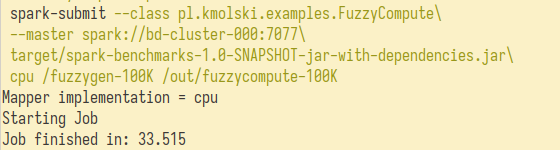
\includegraphics[width=0.8\textwidth]{graf/FuzzyCompute-interface.png}
	\caption{Przykładowe wywołanie programu FuzzyCompute.}
	\label{fig:fuzzycompute:run}
\end{figure}

Formatem plików wejściowych i wyjściowych dla programu jest SequenceFile.

\subsection{Program FuzzyFilter}

Ostatni z omawianych programów testowych implementuje filtrowanie rekordów z plików CSV przy użyciu
zbiorów rozmytych. Filtrowanie danych z użyciem zbiorów rozmytych polega na zastosowaniu logiki
rozmytej do określenia stopnia przynależności elementów, a następnie usunięciu rekordów, których
stopień przynależności znajduje się poniżej ustawionego progu.

Tradycyjne metody klasyfikacji przyjmują, że obiekt należy do jednej konkretnej klasy. W podejściu
opartym na zbiorach rozmytych obiekt może należeć do wielu klas jednocześnie z różnym stopniem
przynależności. Pozwala to na lepsze uwzględnienie niepewności i niejednoznaczności w danych,
dzięki czemu klasyfikacja jest bardziej elastyczna i lepiej odwzorowuje rzeczywistość.

Funkcje przynależności dla zbiorów rozmytych mogą przyjmować różne kształty, które pozwalają na opisanie
stopnia przynależności w zależności od charakteru danych i problemu. Oto kilka najpopularniejszych
typów funkcji przynależności \cite{fuzzy-sets}:
\begin{itemize}
	\item funkcja impulsowa -- funkcja ta ma wartość 1 dla konkretnego punktu w zbiorze uniwersalnym i
	      0 dla wszystkich innych punktów,
	\item funkcja trójkątna -- określona przez trzy punkty: punkt początkowy, punkt szczytowy i
	      punkt końcowy. Wartość funkcji przynależności wzrasta liniowo od punktu początkowego do punktu
	      szczytowego, a następnie maleje liniowo do punktu końcowego,
	\item funkcja trapezoidalna -- podobna do funkcji trójkątnej, ale z dodatkowym płaskim segmentem dla
	      wartości 1. Zdefiniowana jest przez cztery punkty: punkt początkowy, punkt początku segmentu
	      płaskiego, punkt końca segmentu płaskiego i punkt końcowy,
	\item funkcja Gaussa -- funkcja dzwonowa zdefiniowana przez średnią i odchylenie standardowe.
	      Pozwala na modelowanie stopniowej przynależności, która jest maksymalna w środku i maleje w
	      kierunku wartości krańcowych.
\end{itemize}

Program pozwala na definiowanie relacji przynależności na podstawie funkcji trapezoidalnej. Zaletą tej
funkcji jest jej elastyczność w modelowaniu różnych relacji przynależności. W zależności od wybranych punktów,
określających kształt trapezu, można osiągnąć różne kształty funkcji przynależności.

Ponieważ funkcja trójkątna jest specyficznym przypadkiem funkcji trapezoidalnej, użytkownik może zdefiniować
ją poprzez podanie takich samych wartości dla obu punktów definiujących segment płaski trapezu. Podobne
rozwiązanie umożliwia określenie funkcji impulsowej. Podanie tej samej wartości dla wszystkich parametrów
trapezu powoduje, że powstała funkcja przyjmuje wartość 1 tylko dla jednego punktu.

Podana przez użytkownika lista trapezoidalnych funkcji przynależności jest łączona za pomocą T-normy,
która reprezentuje operację koniunkcji w~dziedzinie zbiorów rozmytych. Przykładowe T-normy to minimum,
produkt algebraiczny oraz norma Łukasiewicza. W programie wykorzystano najprostszą z~nich, czyli
T-normę minimum, która dla dwóch stopni przynależności \( a \) i \( b \) z~zakresu [0, 1] jest
określana przez wzór \ref{eq:fuzzy-tnorm}.

\begin{equation}
    T_{\text{min}}(a, b) = \min(a, b)
    \label{eq:fuzzy-tnorm}
\end{equation}

T-norma minimum ma następujące właściwości:
\begin{itemize}
    \item monotoniczność -- minimum jest funkcją monotoniczną. Oznacza to, że jeżeli mamy dwie pary liczb,
          gdzie \( a \leq c \) i \( b \leq d \), to zawsze \( T_{\text{min}}(a, b) \leq T_{\text{min}}(c, d) \),
    \item idempotentność -- T-norma minimum jest idempotentna, co w praktyce oznacza, że \( T_{\text{min}}(a, a) \)
          zawsze równa się \( a \) dla dowolnej liczby \( a \),
    \item element neutralny --  dla funkcji minimum elementem neutralnym jest liczba 1. Innymi słowy,
          \( T_{\text{min}}(a, 1) \) zawsze równa się \( a \) dla dowolnego \( a \) z przedziału [0, 1],
    \item komutatywność -- oznacza to, że funkcja minimum zwraca ten sam wynik niezależnie od kolejności
          argumentów, czyli \( T_{\text{min}}(a, b) \) jest równa \( T_{\text{min}}(b, a) \)
          dla dowolnych liczb \( a \) i \( b \),
    \item łączność -- funkcja minimum jest również łączna. W praktyce oznacza to, że dla dowolnych
          liczb \( a \), \( b \) i \( c \) z przedziału [0, 1], \( T_{\text{min}}(a, T_{\text{min}}(b, c)) \)
          jest równa \( T_{\text{min}}(T_{\text{min}}(a, b), c) \).
\end{itemize}

Program dla platformy Spark wykorzystuje moduł Spark SQL, który został wybrany ze względu na zdolność
do operowania na plikach CSV bez definiowania schematu danych. Umożliwia to przetwarzanie danych o różnej
strukturze bez konieczności zmiany programu. Rozmyte filtrowanie rekordów jest implementowane przez klasy opisane w załączniku \ref{ch:techdoc}:
\begin{itemize}
    \item CpuFuzzyFilterFunction (listing \ref{ch:cpu-fuzzyfilter-function}) -- implementacja dla procesora głównego,
    \item JcudaFuzzyFilterFunction (listing \ref{ch:jcuda-fuzzyfilter-function}) -- implementacja używająca algorytmu w języku CUDA.
\end{itemize}

\subsubsection*{Specyfikacja zewnętrzna}

Program Spark oczekuje co najmniej czterech argumentów wiersza poleceń, których przykładowe użycie
zostało przedstawione na rysunku \ref{fig:fuzzyfilter:run}:
\begin{itemize}
	\item \lstinline{mapper} -- implementacja algorytmu (jeden z "cpu" lub "cuda"),
	\item \lstinline{inputFile} -- plik wejściowy w formacie CSV,
	\item \lstinline{outputFile} -- ścieżka pliku w HDFS, do którego zostaną zapisane rekordy,
	\item \lstinline{threshold} -- wartość progowa dla funkcji przynależności rekordu,
    \item \lstinline{filters} -- parametry określające trapezoidalną funkcję przynależności.
\end{itemize}

Składnia parametru \lstinline{filters} składa się z pięciu części:
\begin{itemize}
	\item punktu początkowego,
	\item punktu początku segmentu płaskiego,
	\item punktu końca segmentu płaskiego,
	\item punktu końcowego,
    \item kolumny, dla której obliczany jest stopień przynależności
\end{itemize}

Program wyświetla w konsoli wybrany algorytm, czas wykonania oraz liczbę rekordów spełniających
zadany warunek. W przypadku braku argumentów lub ich niepoprawności, aplikacja poinformuje użytkownika
o~błędzie i~przedstawi instrukcję właściwego użycia.

\begin{figure}[h]
	\centering
	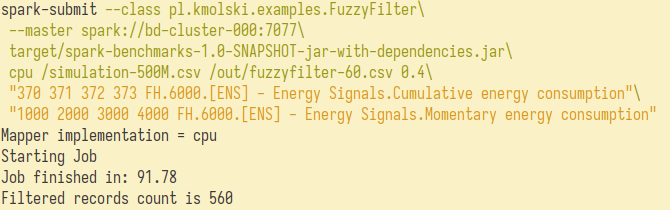
\includegraphics[width=0.8\textwidth]{graf/FuzzyFilter-interface.png}
	\caption{Przykładowe wywołanie programu FuzzyFilter.}
	\label{fig:fuzzyfilter:run}
\end{figure}

Format plików odczytywanych i~zapisywanych przez program FuzzyFilter to CSV.
